\vspace{-6mm}
\section*{1. VANET 시뮬레이션 준비 및 실행 과정}

\subsection*{OpenStreetMap 지도 가져오기}
    OpenStreetMap을 통해 신촌 지역의 지도를 ‘map.osm’ 파일로 다운로드 한다.
    \vspace{-3mm}
    \begin{figure}[!h]\centering 
        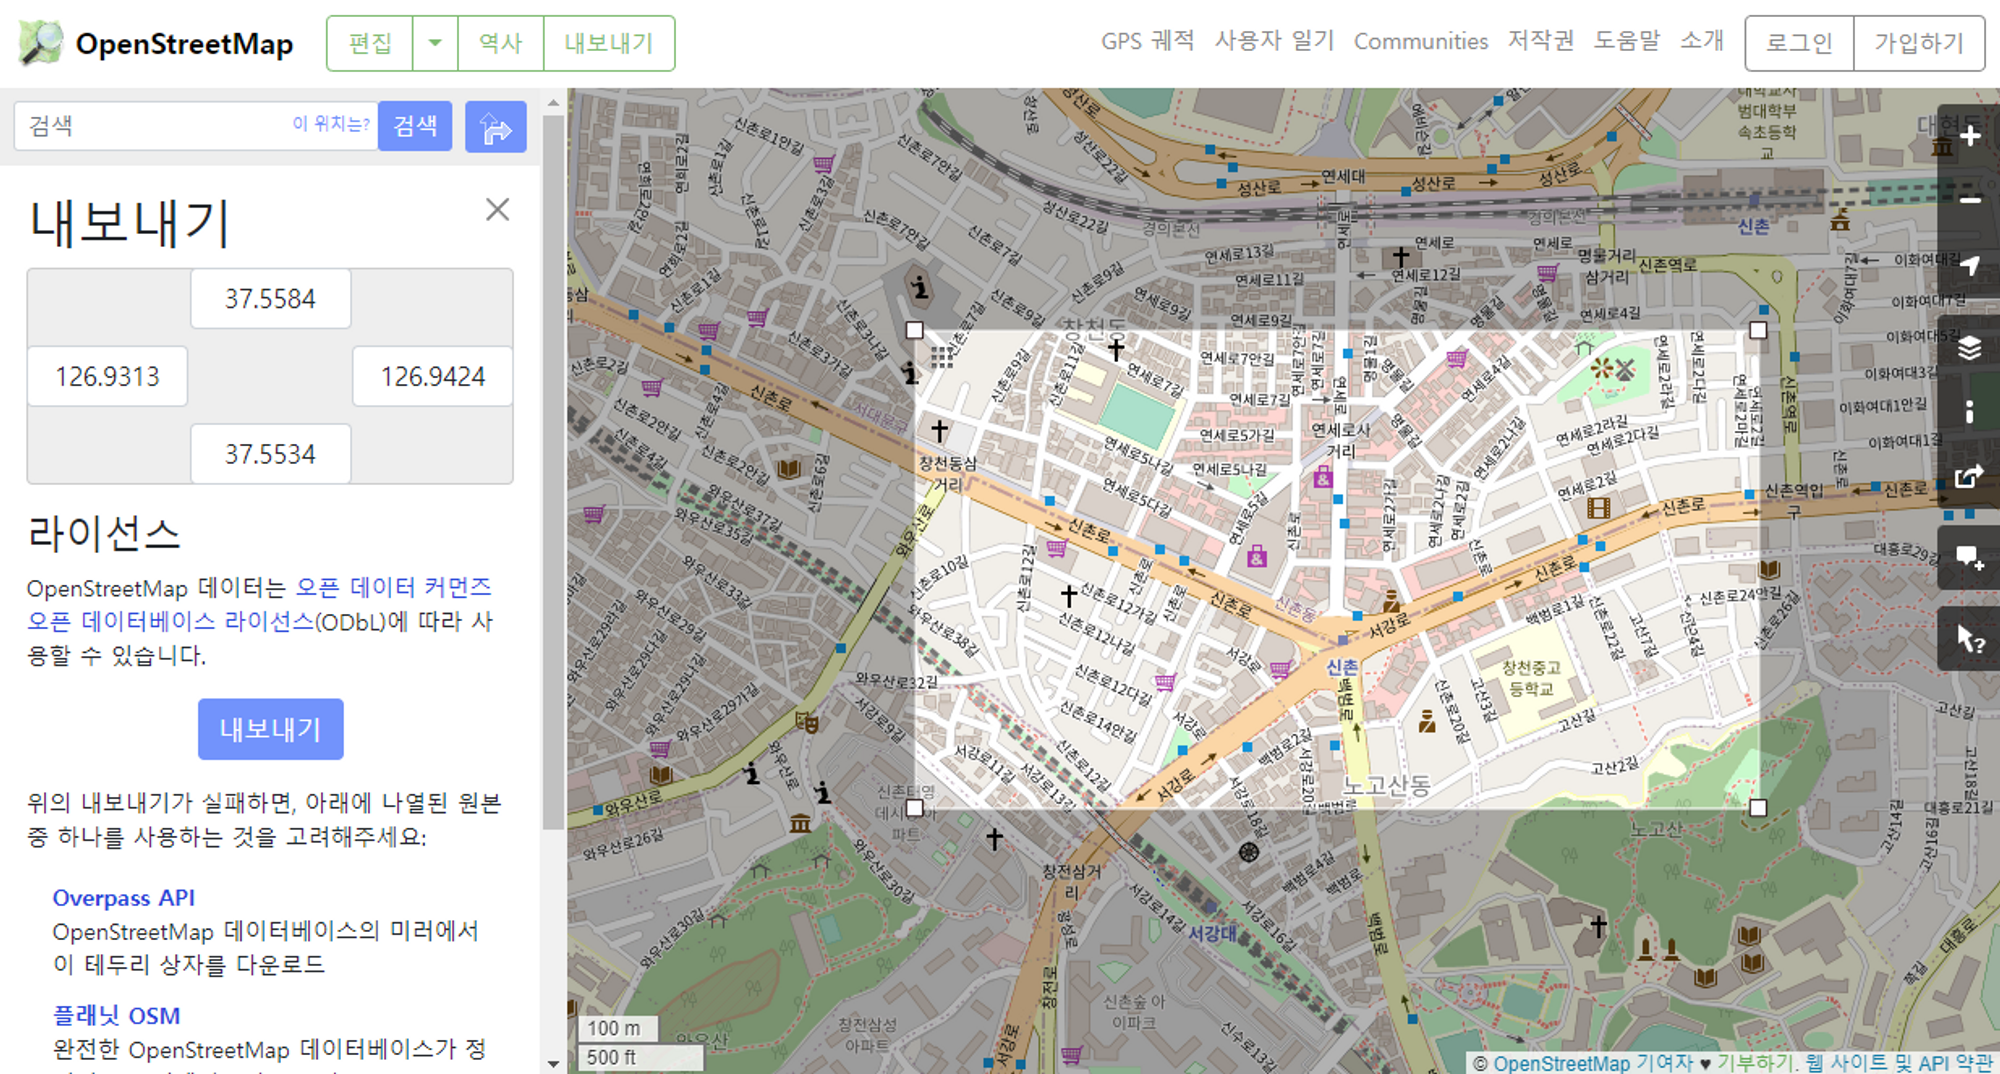
\includegraphics[width=.80\textwidth]{image/week14/1-1.png}
        \caption{\footnotesize
        OpenStreetMap 지도 다운로드}
        \vspace{-10pt}
    \end{figure}
   
\subsection*{SUMO 상에서 map 구현}
    ‘map.osm’ 파일을 이용해 terminal 상에서 ‘2.net.xml’ 파일을 생성한다.
    \vspace{-3mm}
    \begin{figure}[!h]\centering 
        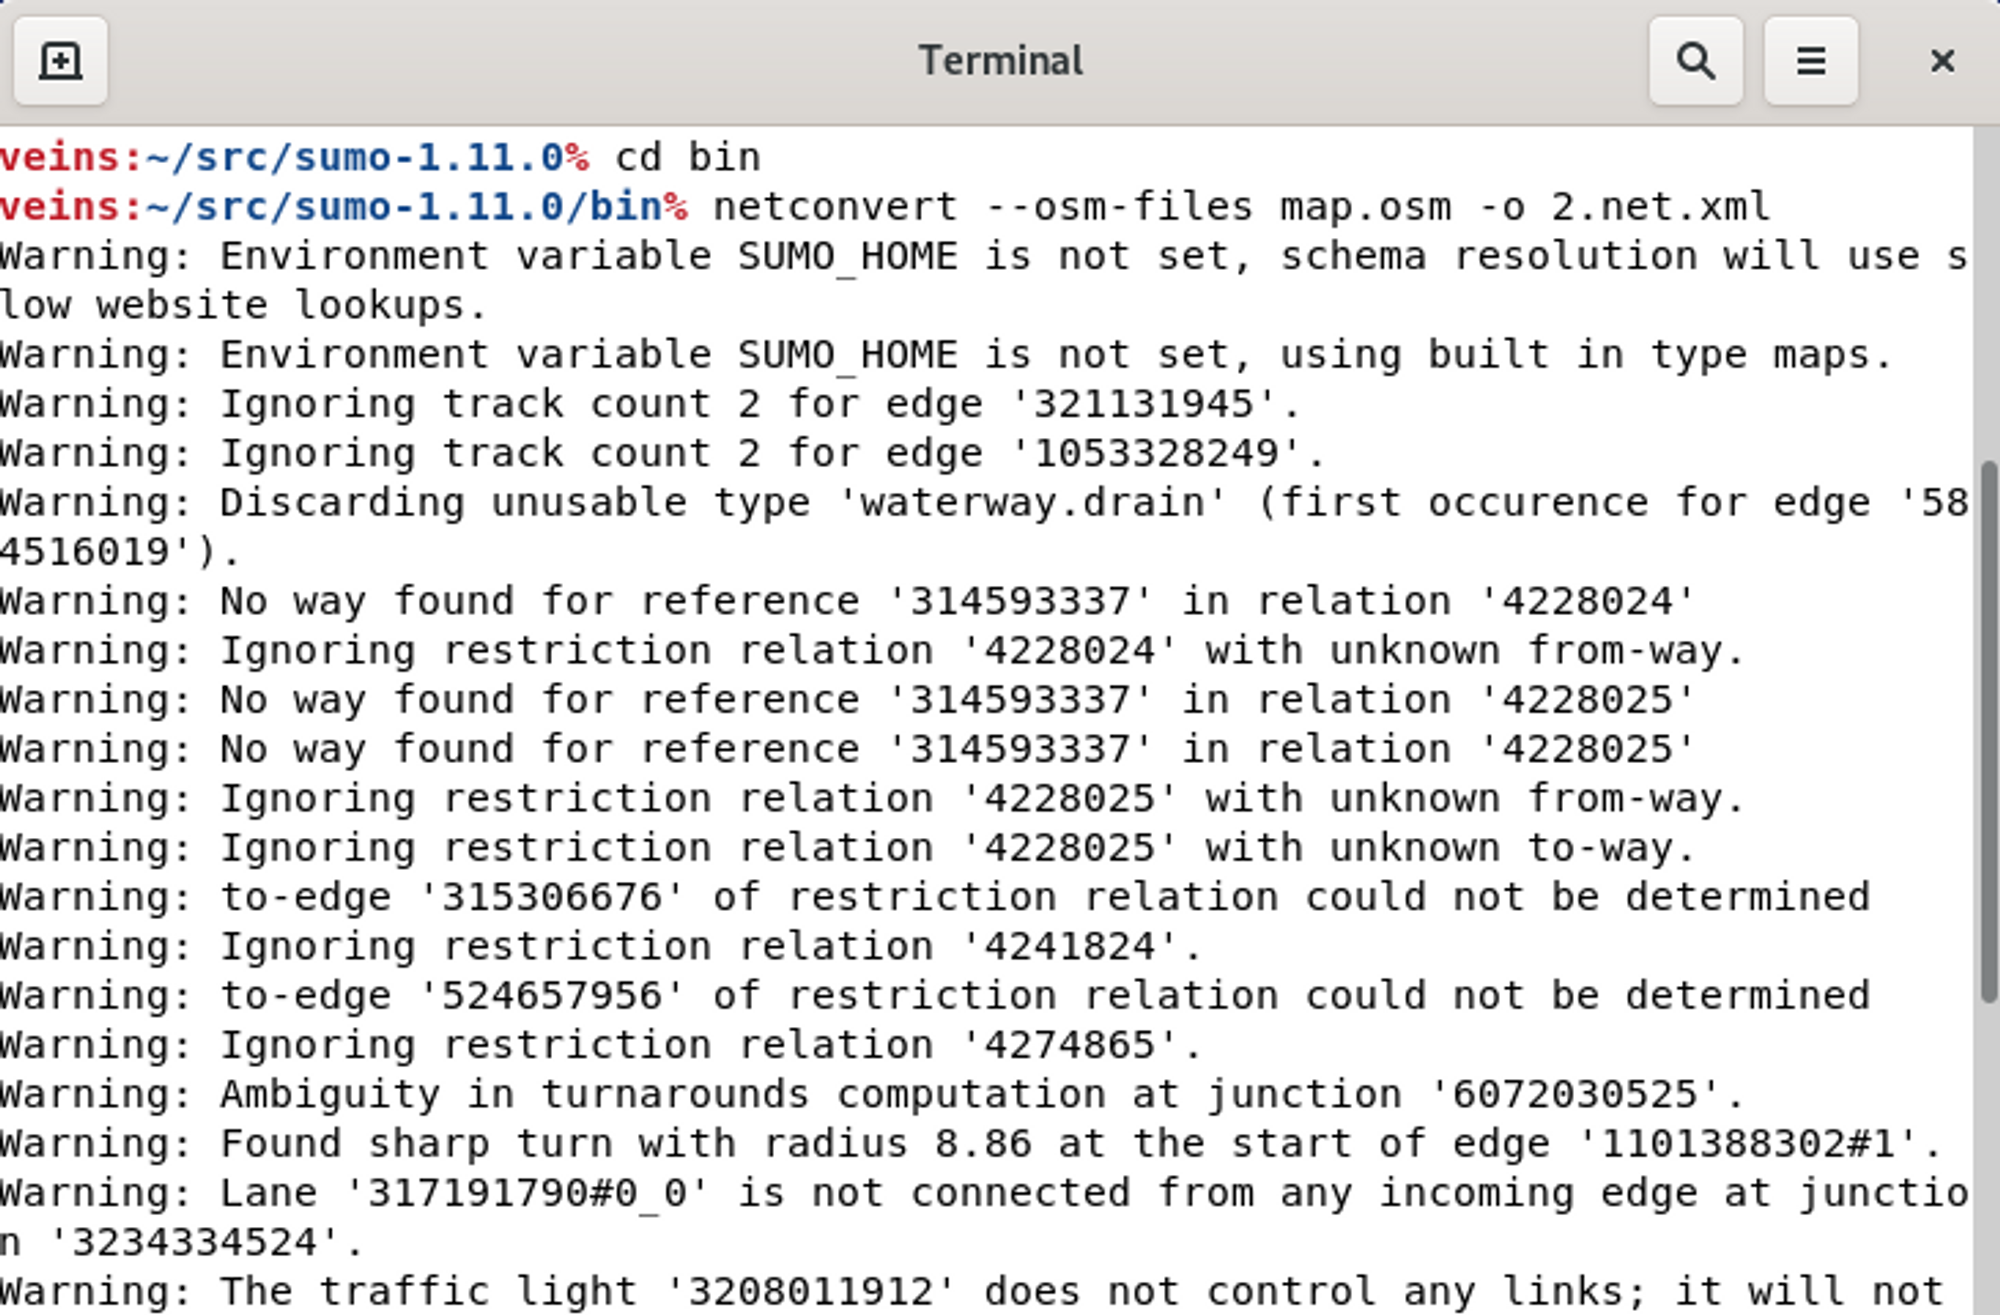
\includegraphics[width=.68\textwidth]{image/week14/1-2.png}
        \caption{\footnotesize
        2.net.xml 파일 생성}
        \vspace{-10pt}
    \end{figure}
\newpage
    
    typemap.xml 파일을 이용해 terminal 상에서 ‘2.poly.xml’ 파일을 생성한다.
    \vspace{-3mm}
    \begin{figure}[!h]\centering 
        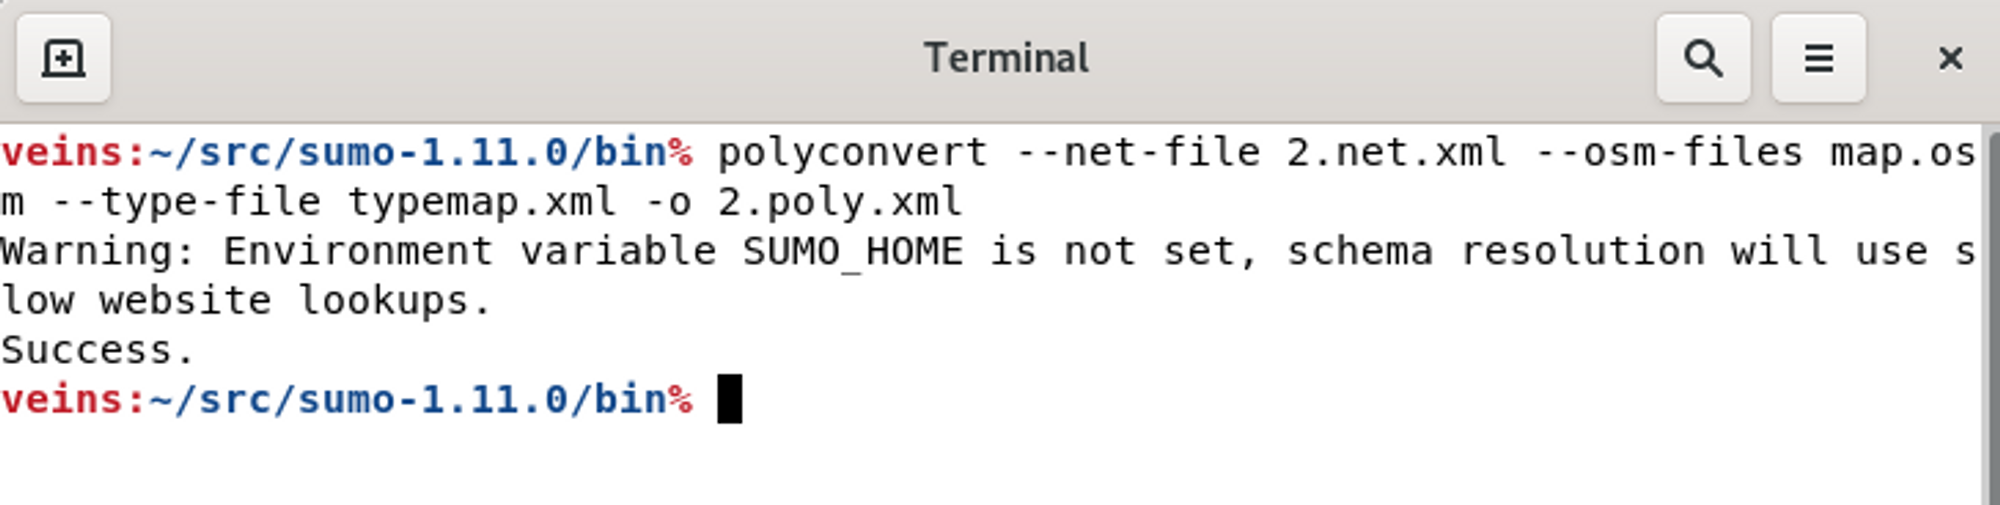
\includegraphics[width=.68\textwidth]{image/week14/1-3.png}
        \caption{\footnotesize
        2.poly.xml 파일 생성}
        \vspace{-10pt}
    \end{figure}

    terminal 상에서 ‘random.Trips.py’ 코드를 이용해 n개의 차량 위치를 랜덤하게 설정한 ‘2.rou.xml’ 파일을 생성한다. 이번 실험에서는 10, 30, 50, 100개의 차량으로 실험을 4번 진행한다.
    \vspace{-3mm}
    \begin{figure}[!h]\centering 
        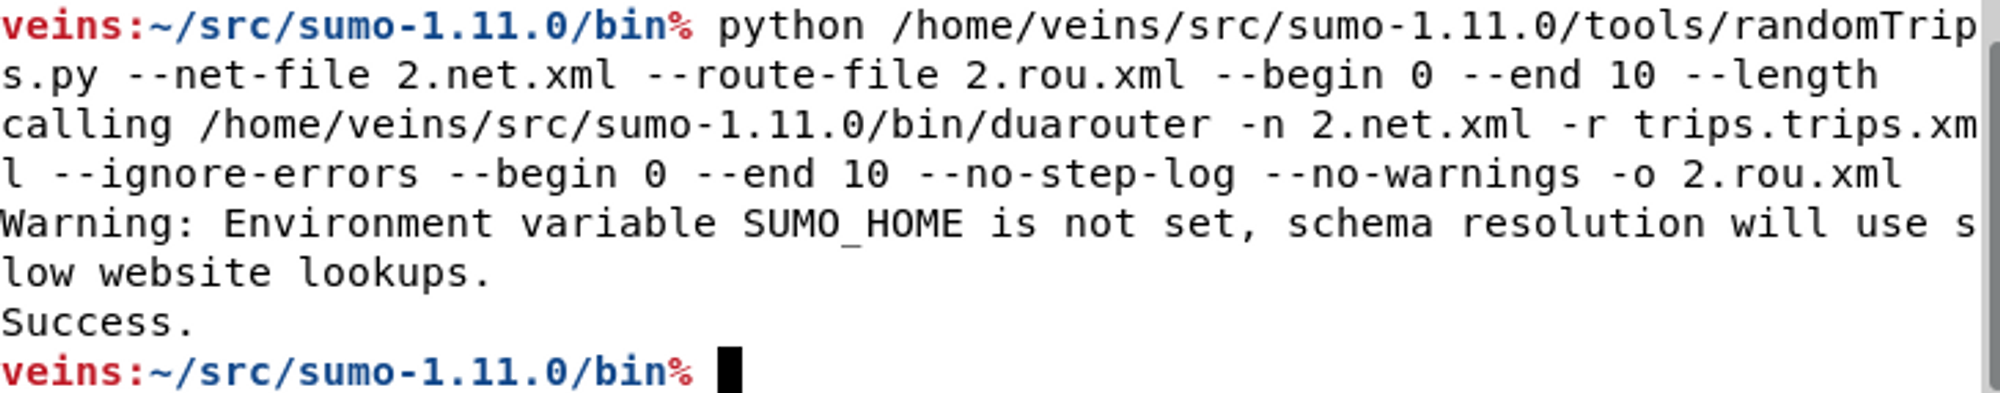
\includegraphics[width=.68\textwidth]{image/week14/1-4.png}
        \caption{\footnotesize
        2.rou.xml 파일 생성}
        \vspace{-10pt}
    \end{figure}
    
    앞서 생성한 ‘2.net.xml’, ‘2.poly.xml’, ‘2.rou.xml’ 파일을 시뮬레이션을 진행할 Home/src/veins/examples/veins 폴더로 이동시킨다. 폴더 내의 ‘erlangen.lauchd.xml’, ‘erlangen.sumo.cfg’ 파일이 이 3개의 파일을 사용하도록 코드를 수정한다.
    \vspace{-3mm}
    \begin{figure}[h!]
        \centering
        \subfloat{
            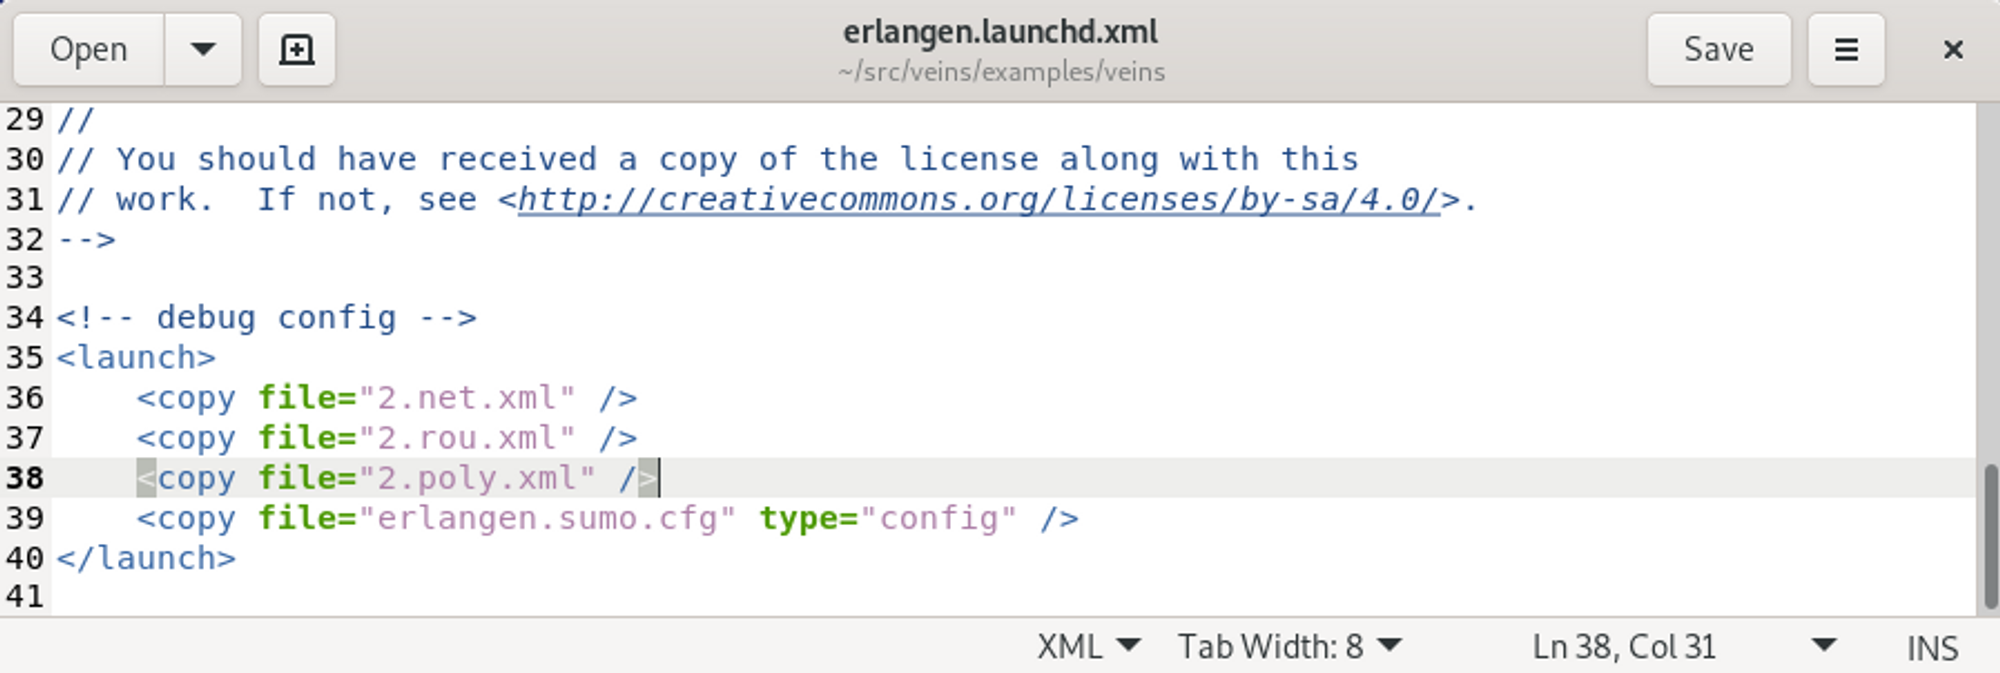
\includegraphics[width=0.46\textwidth]{image/week14/1-5.png}
        }\hspace{3mm}
        \subfloat{
            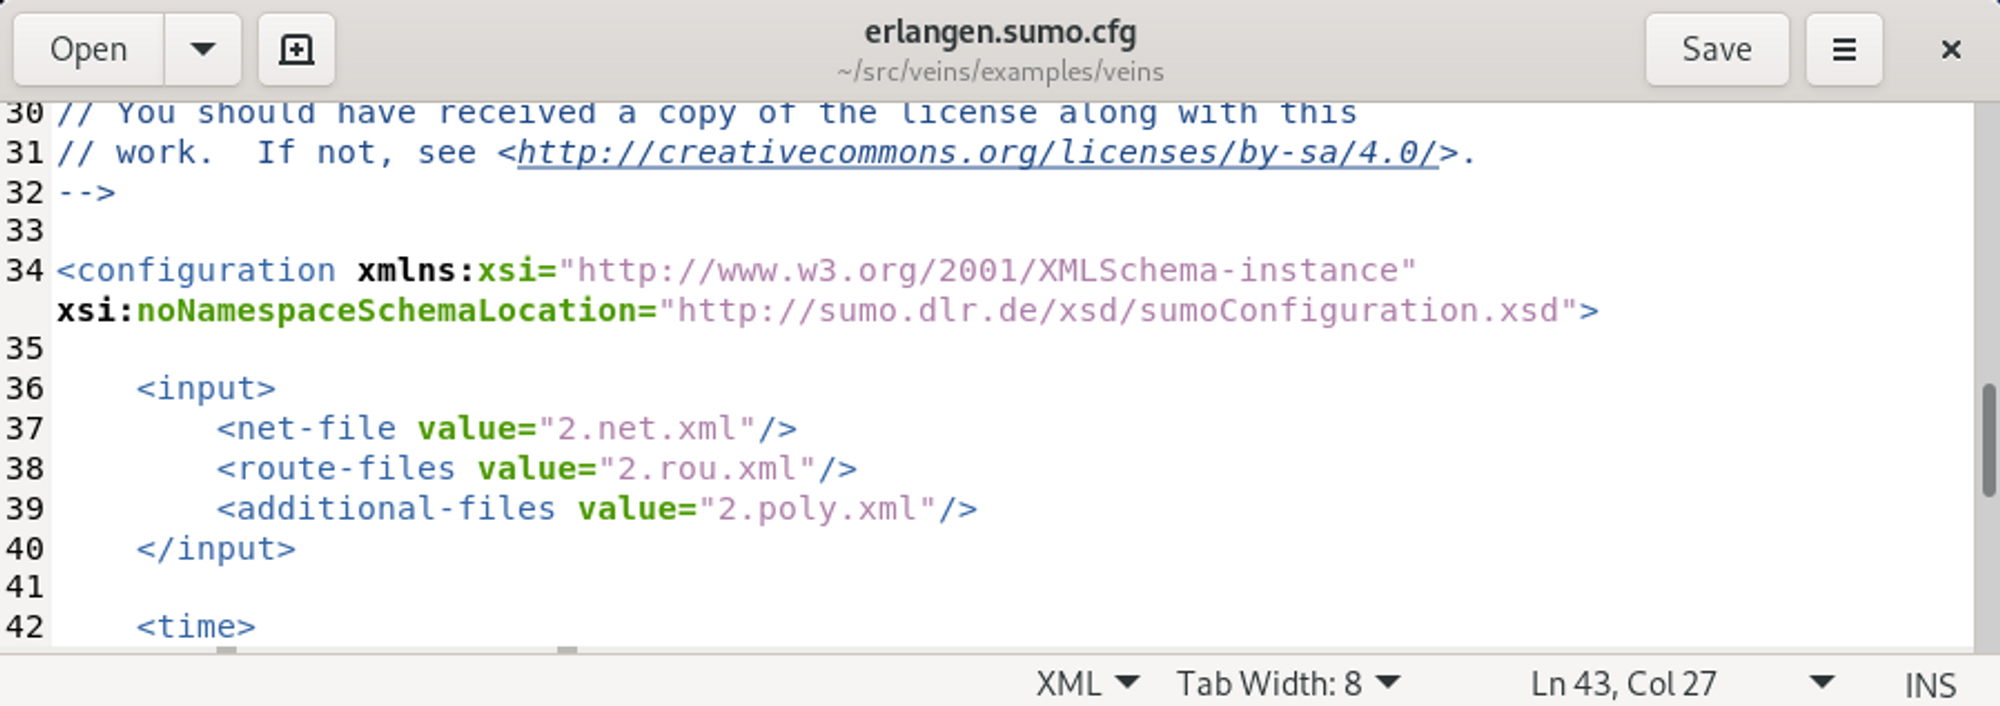
\includegraphics[width=0.46\textwidth]{image/week14/1-6.png}
        }
        \caption{erlangen.lauchd.xml, erlangen.sumo.cfg 파일 수정}
        \vspace{-2mm}
    \end{figure}

\subsection*{omnetpp.ini 파일 수정}
    ‘omnetpp.ini’ 파일의 Mobility 부분을 아래와 같이 수정한다.
    \vspace{-3mm}
    \begin{figure}[!h]\centering 
        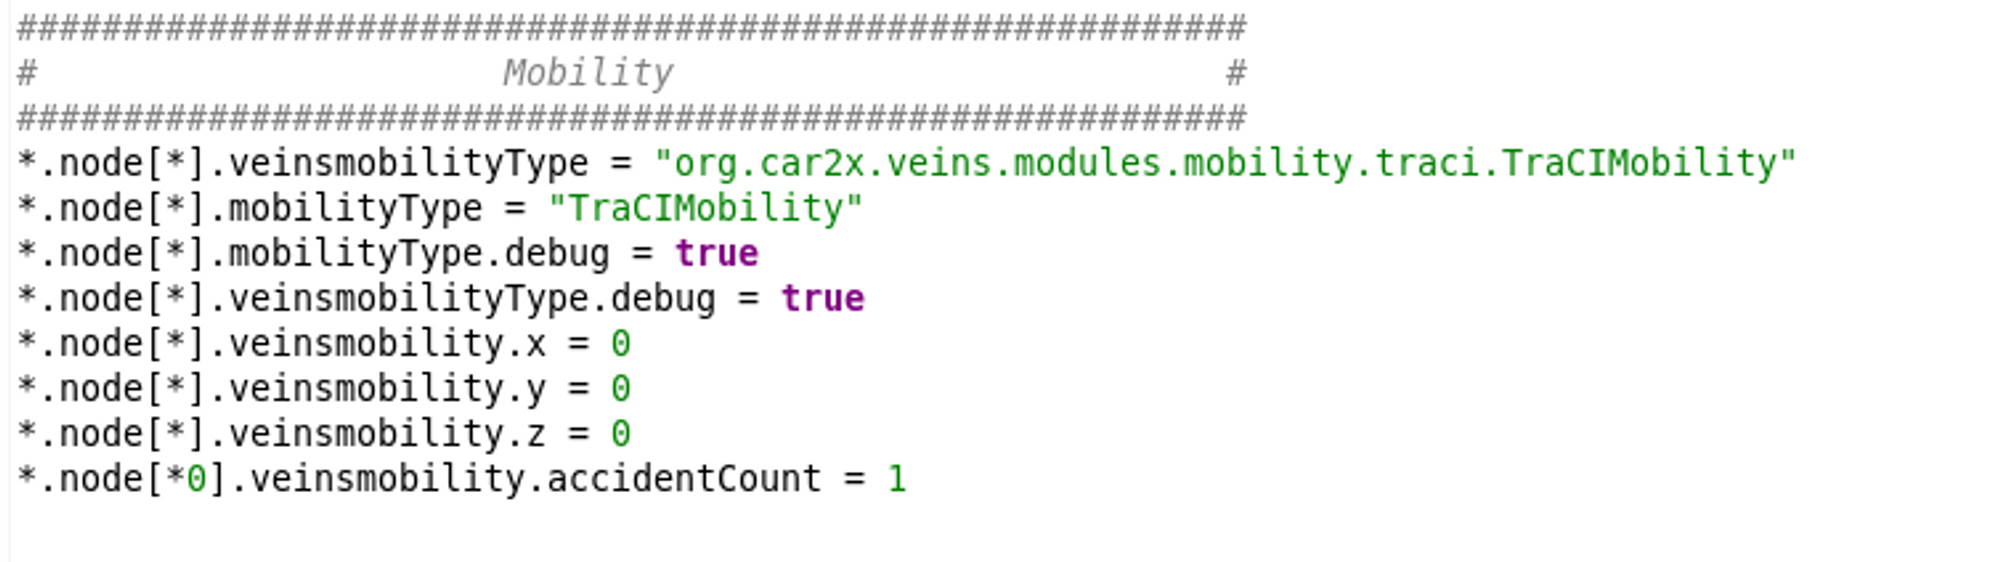
\includegraphics[width=.80\textwidth]{image/week14/1-7.png}
        \caption{\footnotesize
        omnetpp.ini 파일 Mobility 부분}
        \vspace{-10pt}
    \end{figure}

    이번 실험은 RSU 없이 차량간의 V2V 통신만 이용하기 때문에 ‘omnetpp.ini’의 RSU setting 부분과 RSUExampleScenario.ned 파일의 RSU 설정을 지운다.

\newpage
\subsection*{시뮬레이션 실행}
    위의 설정들을 바탕으로 시뮬레이션을 진행했다. 아래의 그림은 차량의 개수를 각각 10, 30, 50, 100개로 설정한 시뮬레이션의 구동 화면이다.
    \vspace{-3mm}
    \begin{figure}[h!]
        \centering
        \subfloat[차량 노드 10개]{
            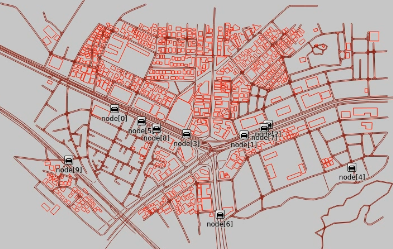
\includegraphics[width=0.46\textwidth]{image/week14/1-8.png}
        }
        \subfloat[차량 노드 30개]{
            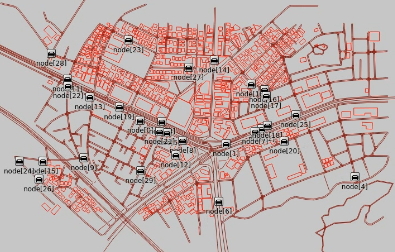
\includegraphics[width=0.46\textwidth]{image/week14/1-9.png}
        }\hspace{3mm}
        \subfloat[차량 노드 50개]{
            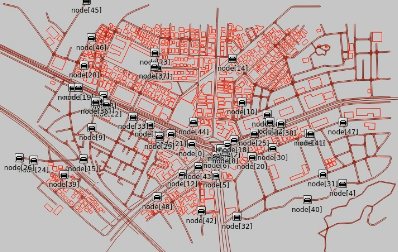
\includegraphics[width=0.46\textwidth]{image/week14/1-10.png}
        }
        \subfloat[차량 노드 100개]{
            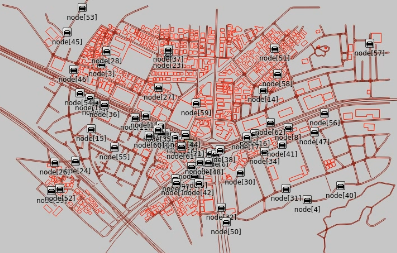
\includegraphics[width=0.46\textwidth]{image/week14/1-11.png}
        }
        \caption{VANET Simulation Result}
        \vspace{-2mm}
    \end{figure}

    OpenStreetMap으로 가져온 신촌 지역의 지도가 시뮬레이션에 적용되어 도로와 건물이 그대로 재현된 것을 확인할 수 있다.
    \vspace{-3mm}
    \begin{figure}[!h]\centering 
        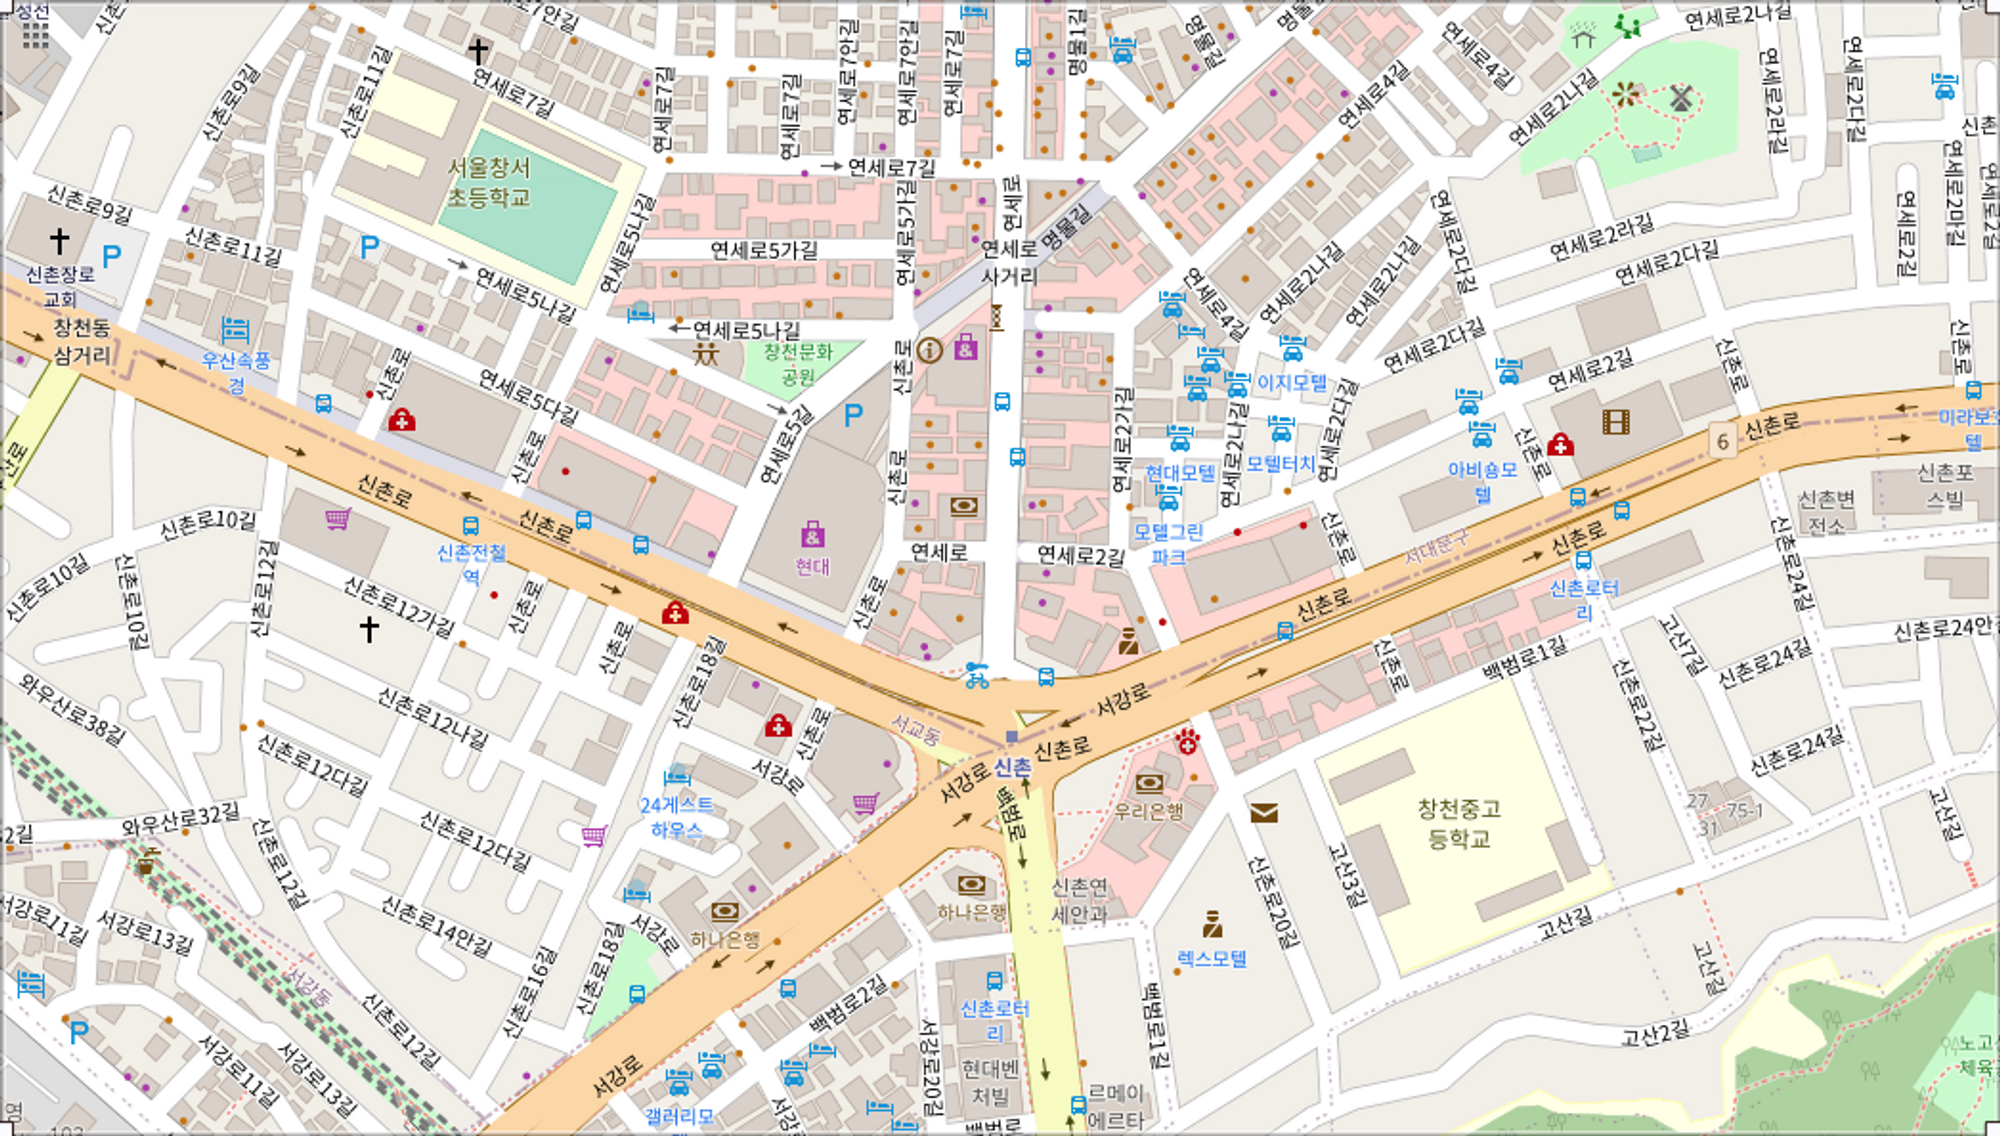
\includegraphics[width=.80\textwidth]{image/week14/1-12.png}
        \caption{\footnotesize
        OpenStreetMap 신촌 지역 지도}
        \vspace{-10pt}
    \end{figure}

%%%%%%%%%%%%%%%%%%%%%%%%%%%%%%%%%%%%%%%%%%%%%%%%%%%%%%%%%%%%%%%%%%%%%%%%%%%%%%%%%%%%%%%%%%%
\clearpage
\section*{2. VANET 시뮬레이션 결과}

\subsection*{차량 노드 [0]의 속도 그래프 비교}
    아래의 그림은 차량의 개수가 각각 10, 30, 50, 100개로 설정한 시뮬레이션의 차량 노드 [0]의 속도 그래프이다. 4개의 시뮬레이션 모두 유사한 속도 그래프를 얻을 수 있었다. 사고 발생으로 정지한 시간만 조금씩 차이가 날뿐 그래프의 모양과 속도의 크기, 전체 시간은 차이가 거의 없었다. \\
    시뮬레이션 구동 화면을 분석한 결과, 차량 노드 [0]의 생성 위치와 경로가 모두 같았다. 생성 위치와 경로가 같기 때문에 그래프의 모양이 유사한 것이다. 차량 노드의 위치와 경로를 생성하는 ‘random.Trips.py’의 랜덤 시드가 고정되어 있기 때문에 각 시뮬레이션의 첫 번째 차량인 차량 노드 [0]의 위치와 경로가 모두 똑같이 생성된 것으로 보인다. \\
    또, 시뮬레이션 진행중에 교통 체증을 거의 볼 수 없었는데, 시뮬레이션에 사용된 지도의 도로 폭이 넓고 우회할 수 있는 경로가 많기 때문으로 보인다. 차량 노드 100개까지는 교통 체증 없이 충분히 수용할 수 있었다. 이러한 이유로 차량 속도의 크기와 목적지 도달 시간이 유사했다.
    \vspace{-3mm}
    \begin{figure}[h!]
        \centering
        \subfloat[차량 노드 10개]{
            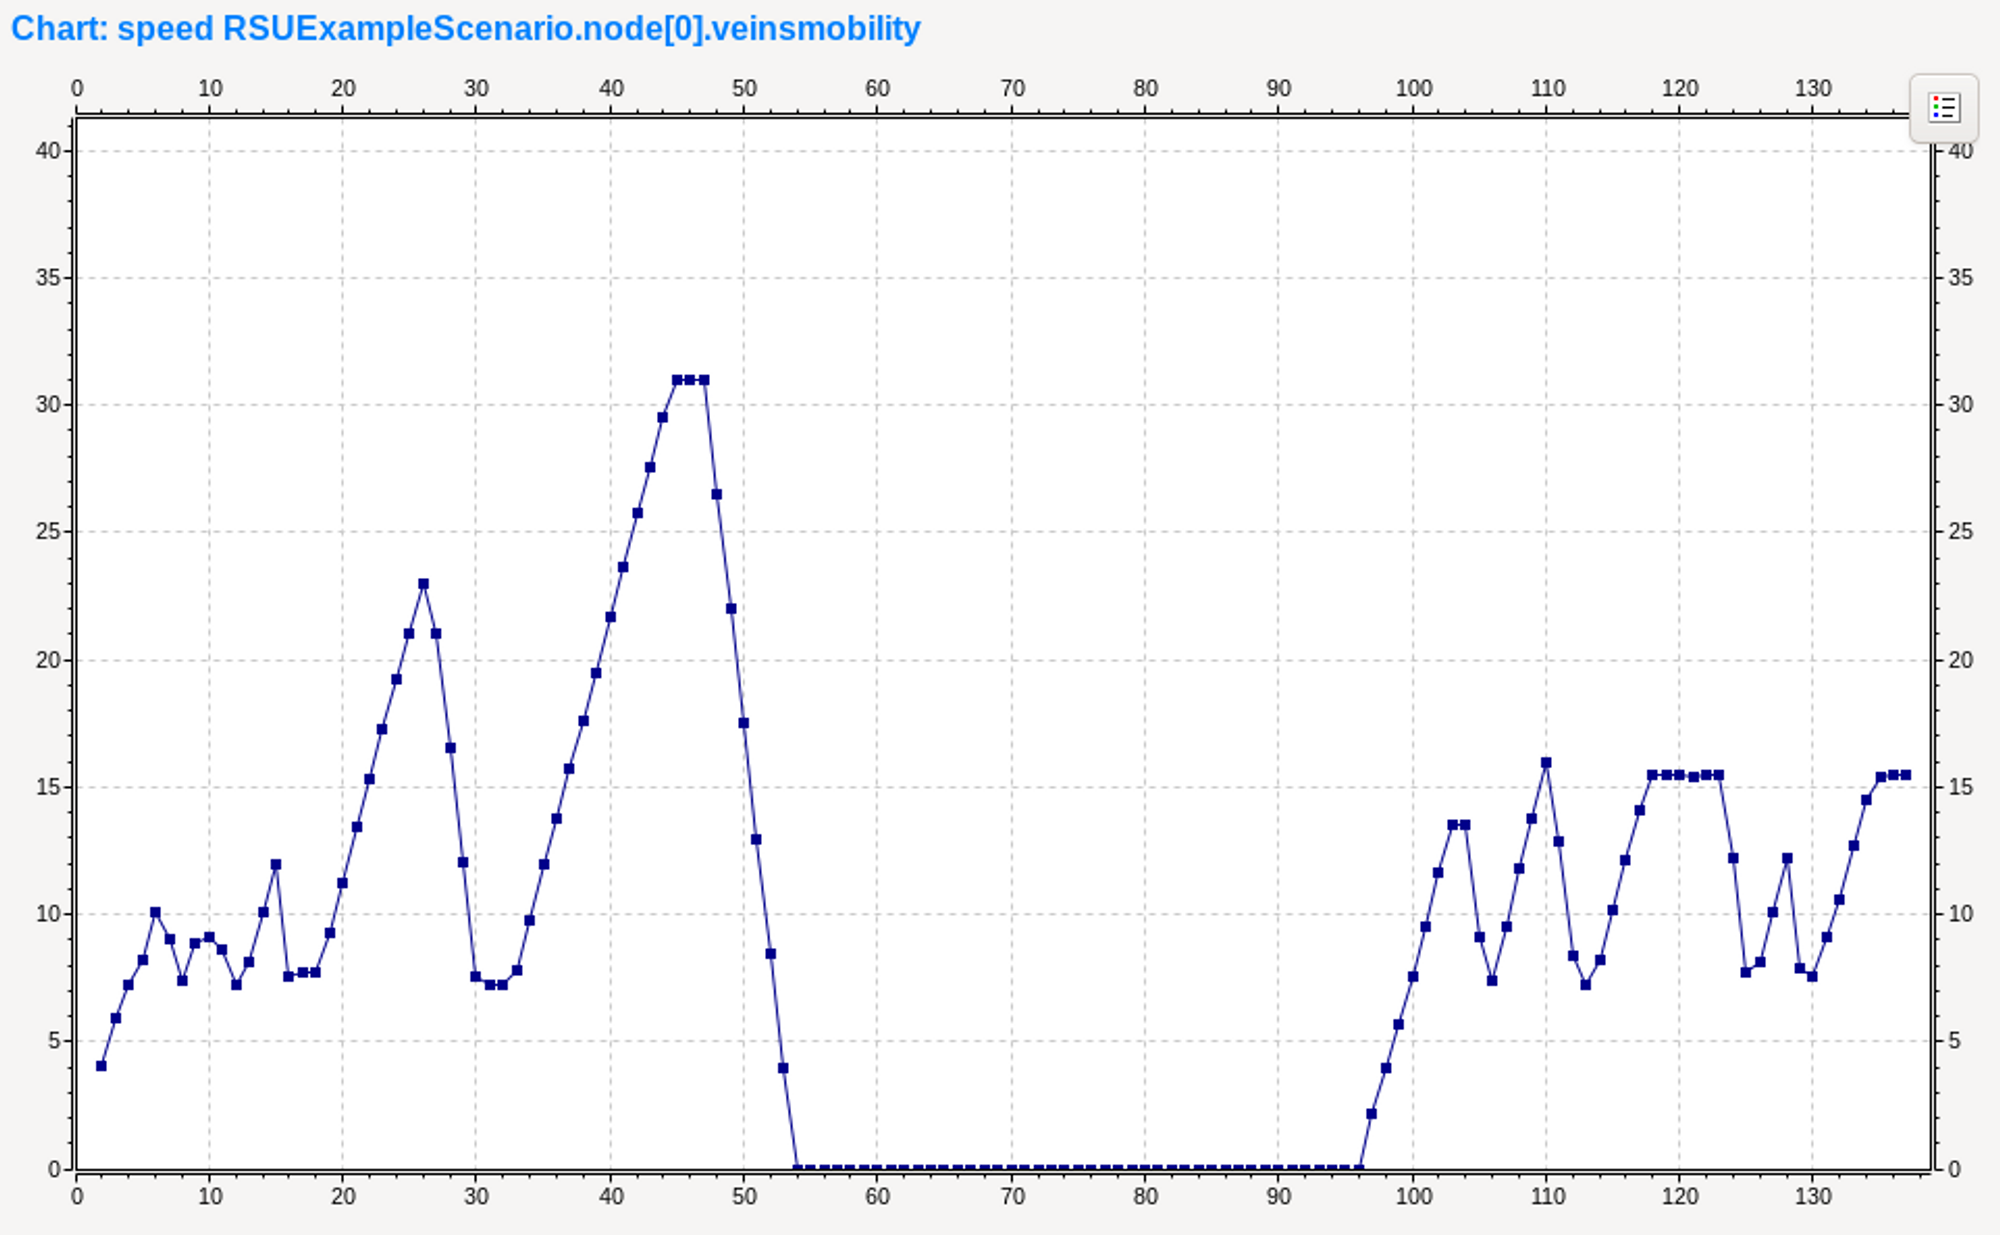
\includegraphics[width=0.46\textwidth]{image/week14/2-1.png}
        }
        \subfloat[차량 노드 30개]{
            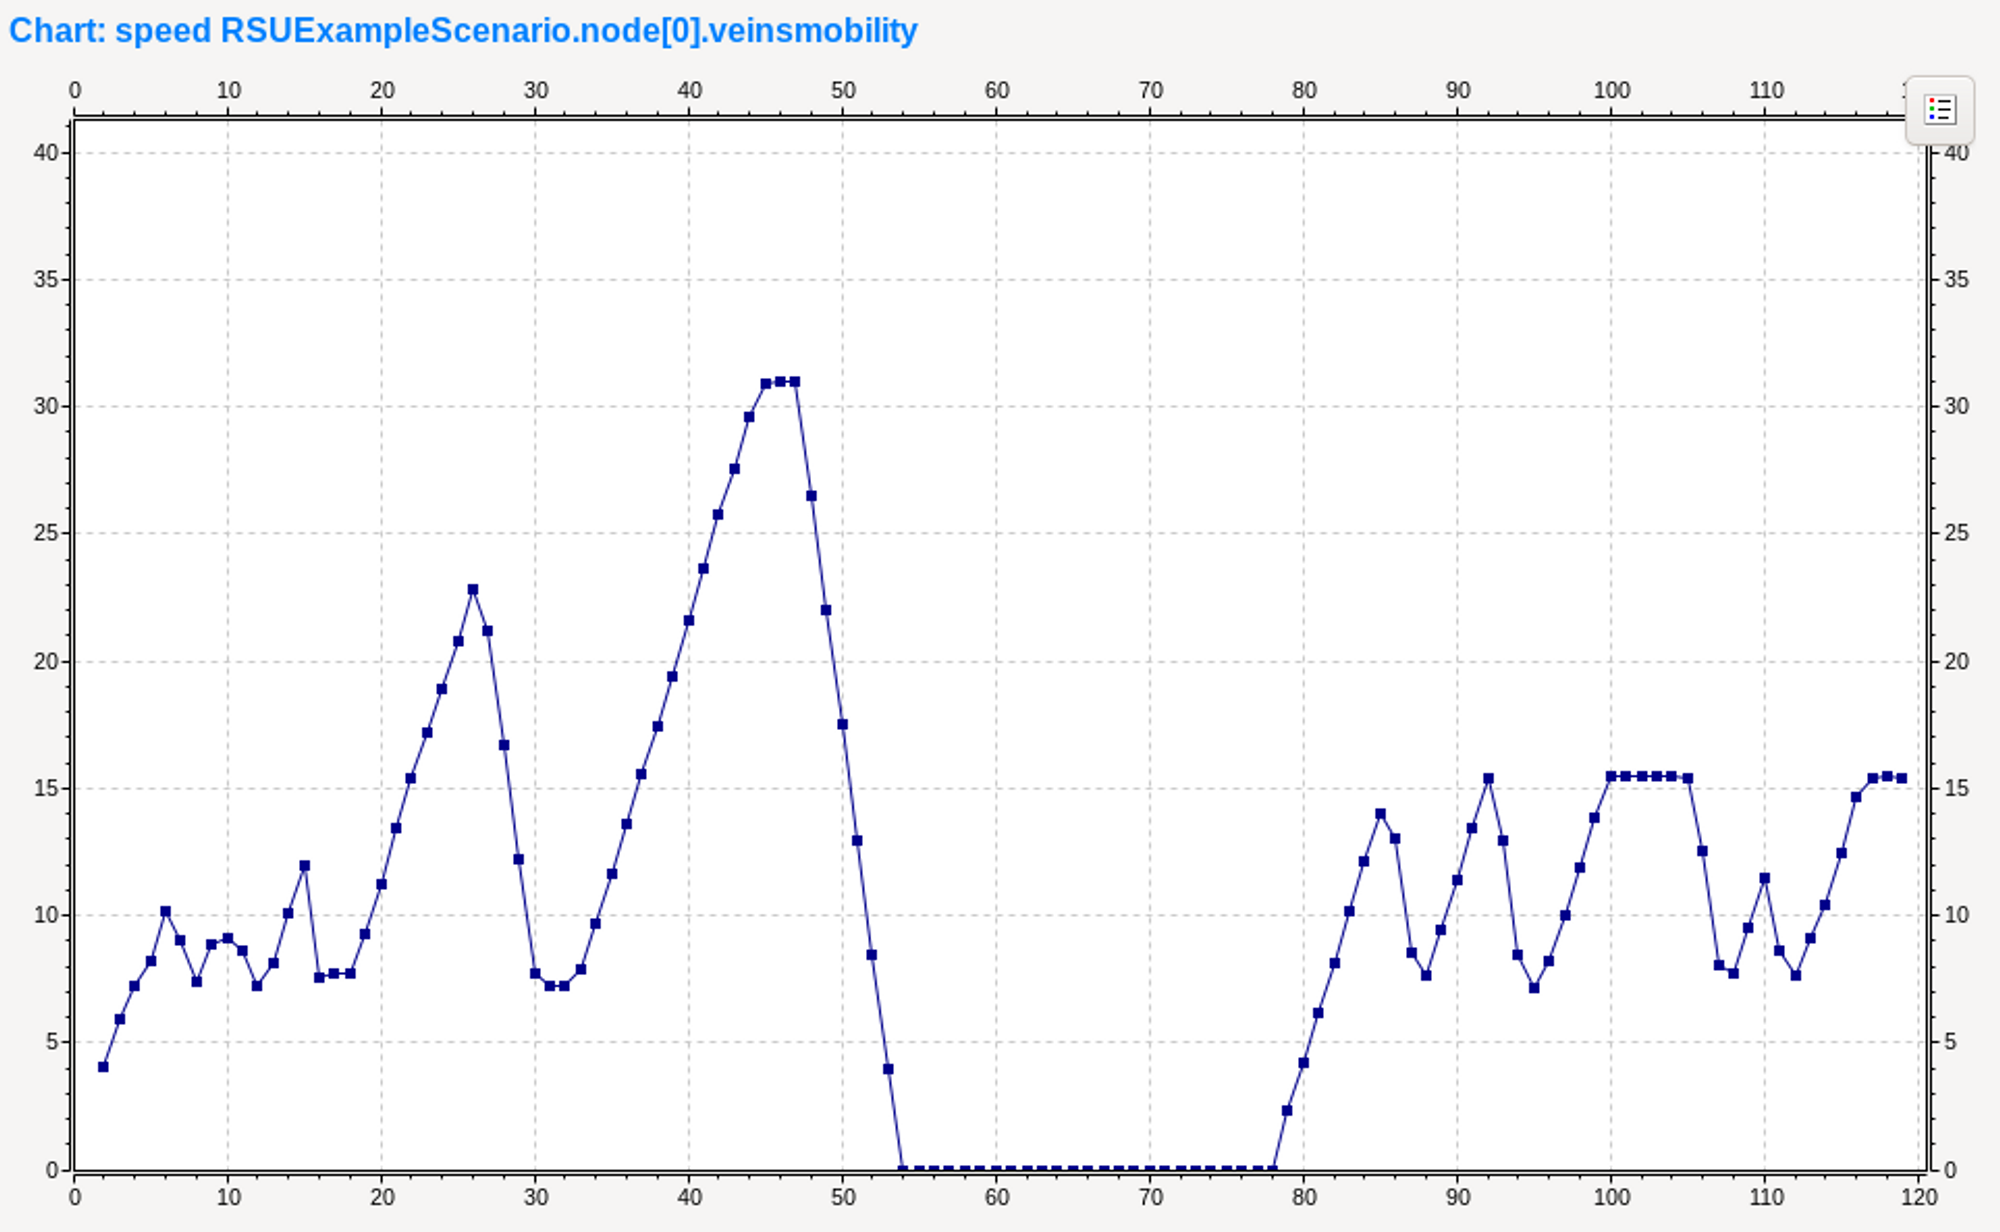
\includegraphics[width=0.46\textwidth]{image/week14/2-2.png}
        }\hspace{3mm}
        \subfloat[차량 노드 50개]{
            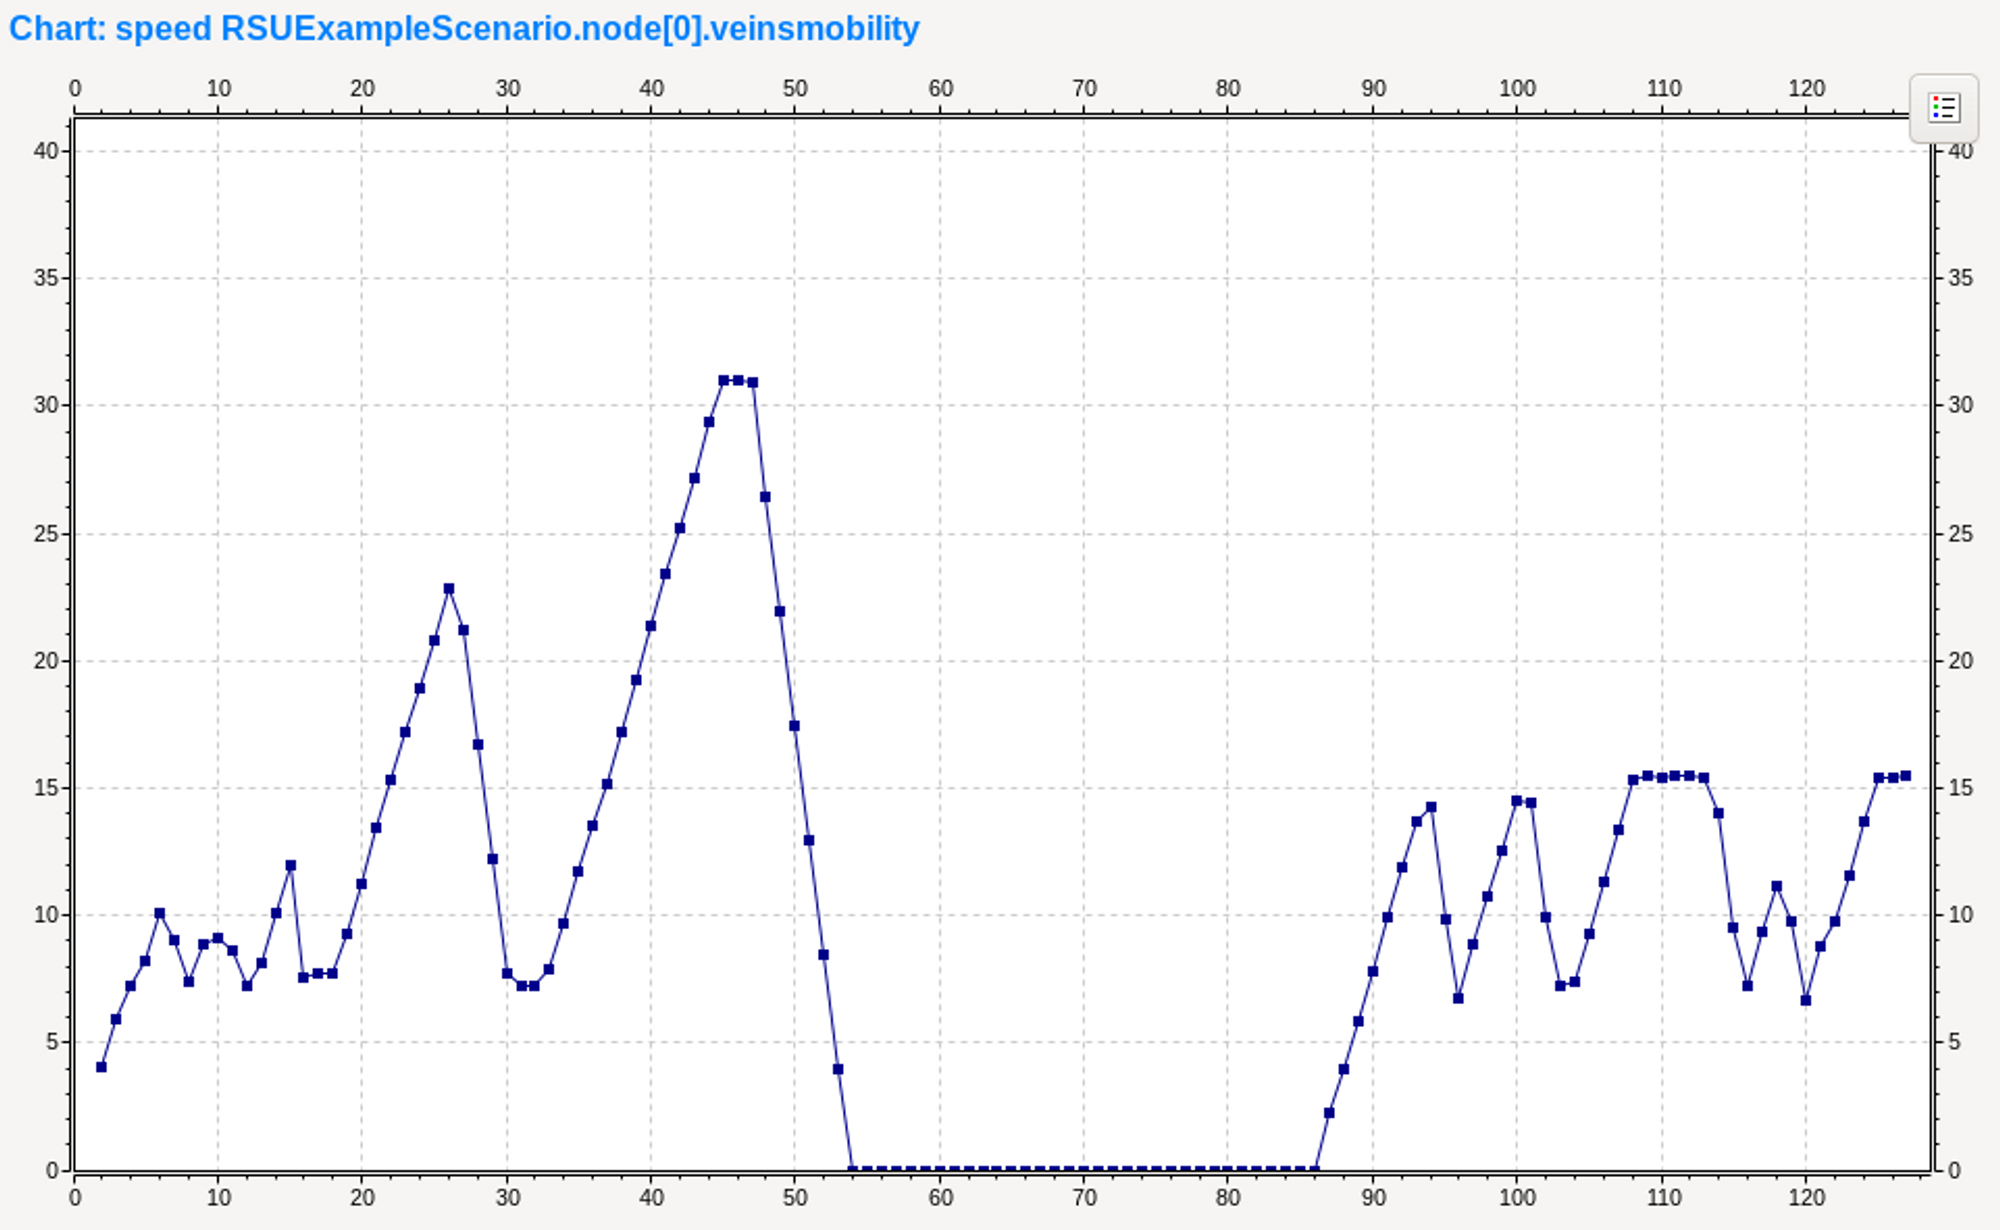
\includegraphics[width=0.46\textwidth]{image/week14/2-3.png}
        }
        \subfloat[차량 노드 100개]{
            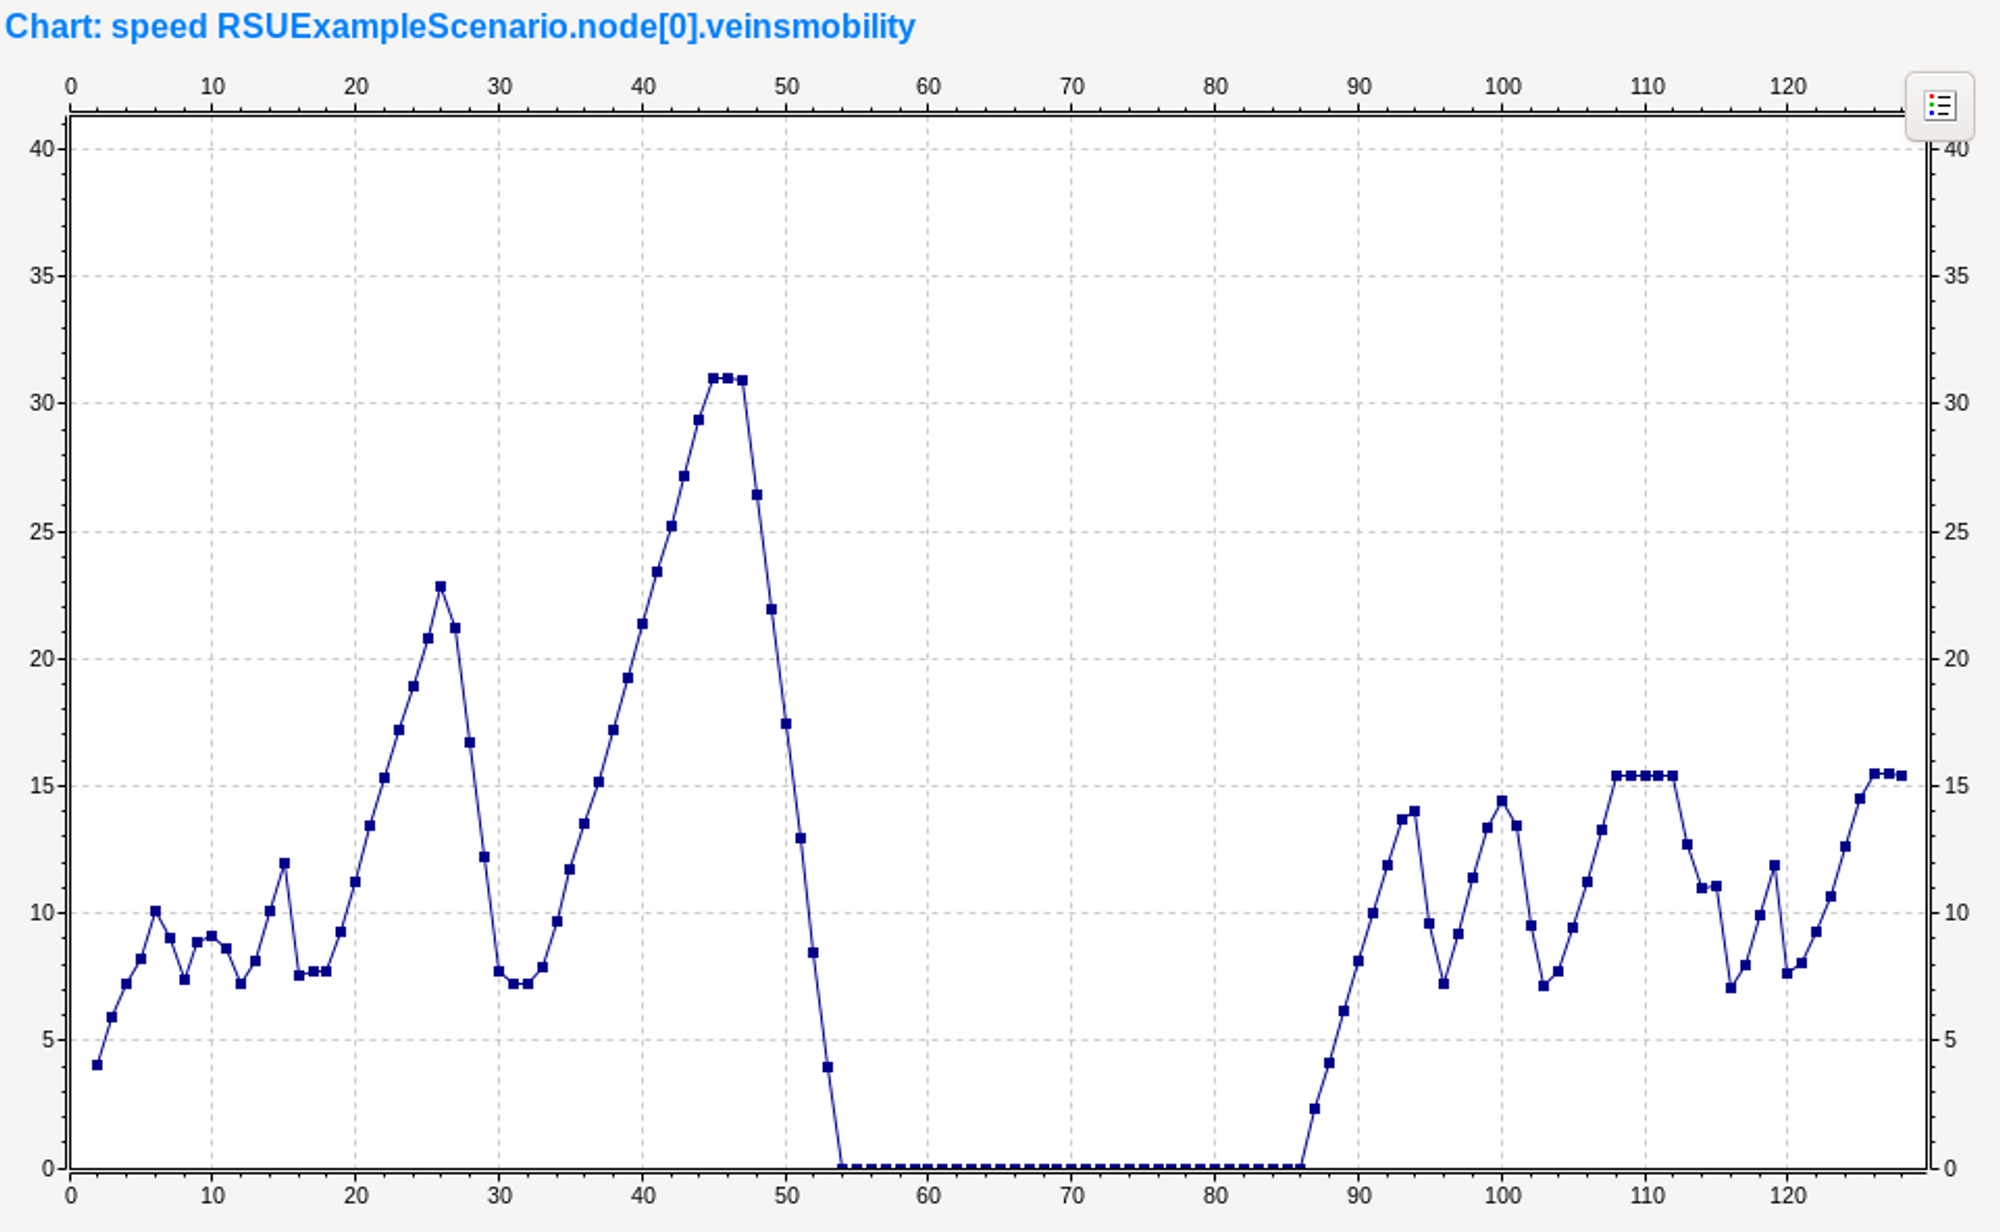
\includegraphics[width=0.46\textwidth]{image/week14/2-4.png}
        }
        \caption{차량 노드 [0]의 속도 그래프}
        \vspace{-2mm}
    \end{figure}

\newpage
\subsection*{전체 차량 노드 개수 대비 Broadcast message을 수신한 차량 노드 개수의 percentage 비교}
    아래의 그림과 같이 시뮬레이션에서 각 차량이 수신한 Broadcast message의 개수를 조사했다. 이를 통해 전체 차량 노드 개수 대비 Broadcast message를 하나 이상 수신한 차량 노드의 개수의 percentage를 구했고, 차량의 개수가 각각 10, 30, 50, 100개로 설정한 4개의 시뮬레이션에 대하여 이 값을 비교했다.
    \vspace{-3mm}
    \begin{figure}[!h]\centering 
        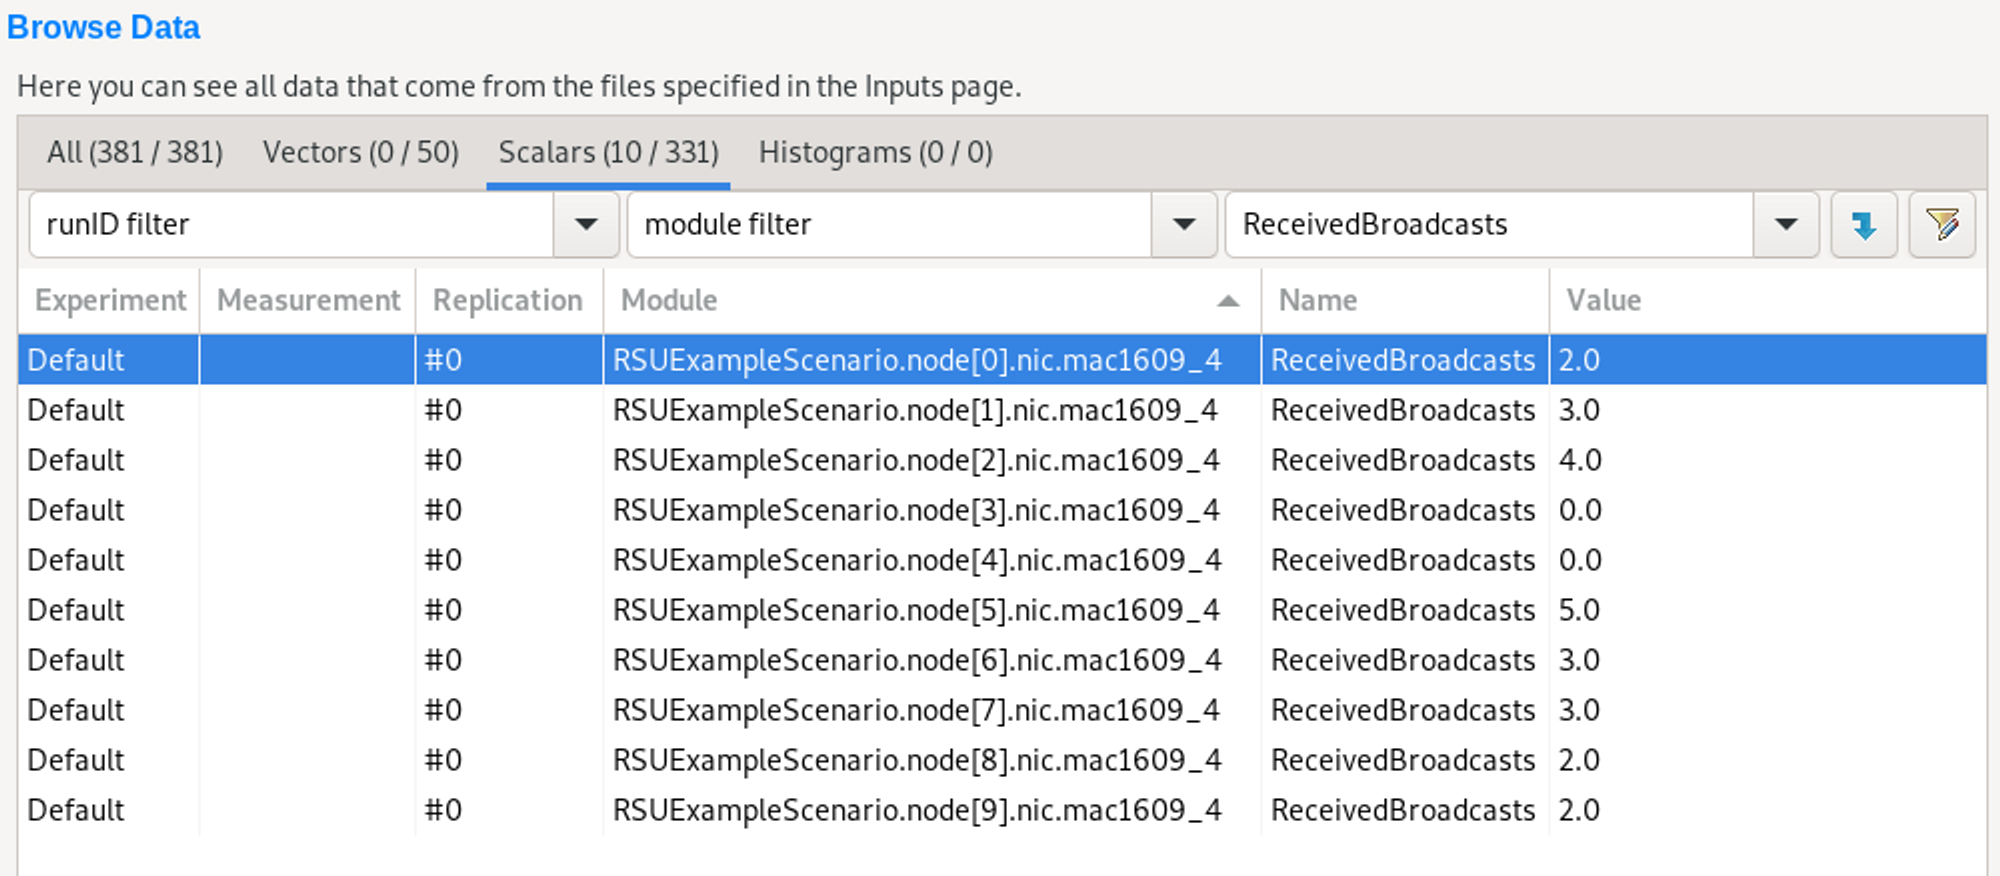
\includegraphics[width=.80\textwidth]{image/week14/2-5.png}
        \caption{\footnotesize
        각 차량이 수신한 Broadcast message의 개수, 차량 노드 10개 시뮬레이션 예시}
        \vspace{-10pt}
    \end{figure}

    4개의 시뮬레이션의 전체 차량 노드 개수 대비 Broadcast message를 수신한 차량 노드의 개수는 뚜렷한 증감 경향성 없이 76\%부터 90\%까지 유사한 결과를 보였다. \\
    지도의 가장자리에 위치해 있거나, 이동 경로가 짧을 경우 Broadcast message를 전혀 수신하지 못하는 경우가 발생하는 것으로 예상되는데, 4개의 시뮬레이션 모두 차량 위치가 랜덤 생성되어 이 비율이 비슷하기 때문에 Broadcast message를 수신한 차량의 비율 역시 유사하게 나온것으로 보인다.
    \vspace{-3mm}
    \begin{table}[h!]
    \centering
        \begin{tabular}{|l|l|l|}
        \hline
        \textbf{차량 노드 개수} & \textbf{Broadcast message 수신한 차량 노드 개수} & \textbf{percentage} \\
        \hline
        10 & 8 & 80\% \\
        \hline
        30 & 23 & 76.7\% \\
        \hline
        50 & 44 & 88\% \\
        \hline
        100 & 90 & 90\% \\
        \hline
        \end{tabular}
        \caption{전체 차량 노드 개수 대비 Broadcast message를 수신한 차량 노드의 개수}
    \end{table}
    \vspace{-3mm}

\newpage
\subsection*{모든 차량 노드의 Total busy time의 합 비교}
    아래의 그림과 같이 시뮬레이션에서 각 차량 노드의 busy time을 조사했다. 이를 통해 모든 차량 노드의 Total busy time을 구했고, 차량의 개수가 각각 10, 30, 50, 100개로 설정한 4개의 시뮬레이션에 대하여 이 값을 비교했다.
    \vspace{-3mm}
    \begin{figure}[!h]\centering 
        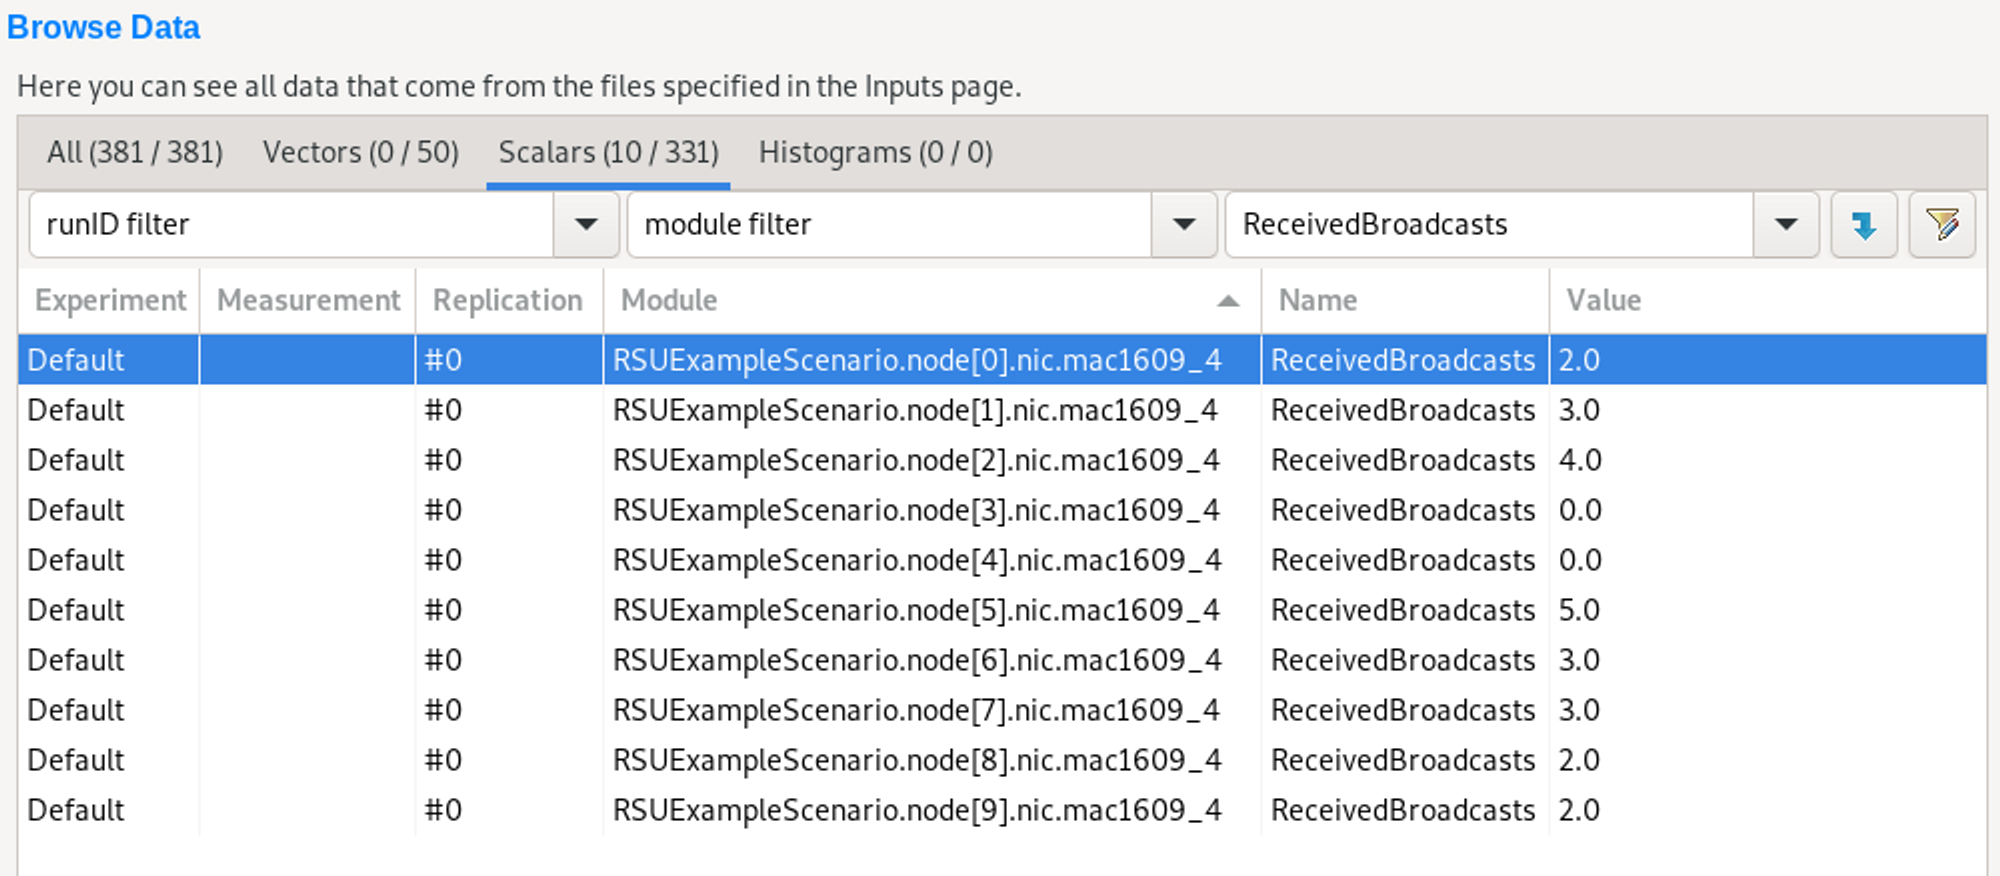
\includegraphics[width=.80\textwidth]{image/week14/2-6.png}
        \caption{\footnotesize
        각 차량의 busy time, 차량 노드 10개 시뮬레이션 예시}
        \vspace{-10pt}
    \end{figure}
    
    4개의 시뮬레이션에서 모든 차량 노드의 Total busy time은 차량 노드 개수가 증가함에 따라 크게 증가했다. \\
    차량 노드의 개수가 많아질수록 Broadcast message를 더 많이 송신하고, Broadcast message를 수신하는 차량도 많아지기 때문에 Total busy time이 증가한다.
    \vspace{-3mm}
    \begin{table}[h!]
    \centering
        \begin{tabular}{|l|l|}
        \hline
        \textbf{차량 노드 개수} & \textbf{Total busy time(s)} \\
        \hline
        10 & 0.0000644 \\
        \hline
        30 & 0.000557 \\
        \hline
        50 & 0.00164 \\
        \hline
        100 & 0.00357 \\
        \hline
        \end{tabular}
        \caption{모든 차량 노드의 Total busy time}
    \end{table}
    \vspace{-3mm}

    